\documentclass[10pt,mathserif]{beamer}
\usepackage{graphicx,amsmath,amssymb,tikz,psfrag}
\usepackage{hyperref}
\usepackage{subcaption}

\usepackage{psfrag,amsfonts,verbatim}
\usepackage{amsthm}
\captionsetup{compatibility=false}


\input defs.tex
\input slide_format.tex

%% begin presentation

\title{\large \bfseries Discovering signals in fMRI data; 
a Bayesian nonparametric approach }

\author{Ahmed Bou-Rabee, Wanrong Zhu, Zheng Xu, Mo Zhou\\[3ex]
STAT 30850\\
University of Chicago}

\date{\today}

\begin{document}

\frame{
\thispagestyle{empty}
\titlepage
}

\section{Introduction}

\begin{frame} {What is fMRI?}
\BIT
\item  fMRI: functional magnetic resonance imaging 
\item  measures the change in brain blood flow while subject is stimulated
\item  data tends to look like (voxel, time, intensity of reading)
\item  e.g., to identify regions of the brain associated with hunger, fMRI readings can be taken while hungry subjects are shown pictures of food.
\EIT
\end{frame}

\begin{frame} {Example}
\begin{figure}
\centering
  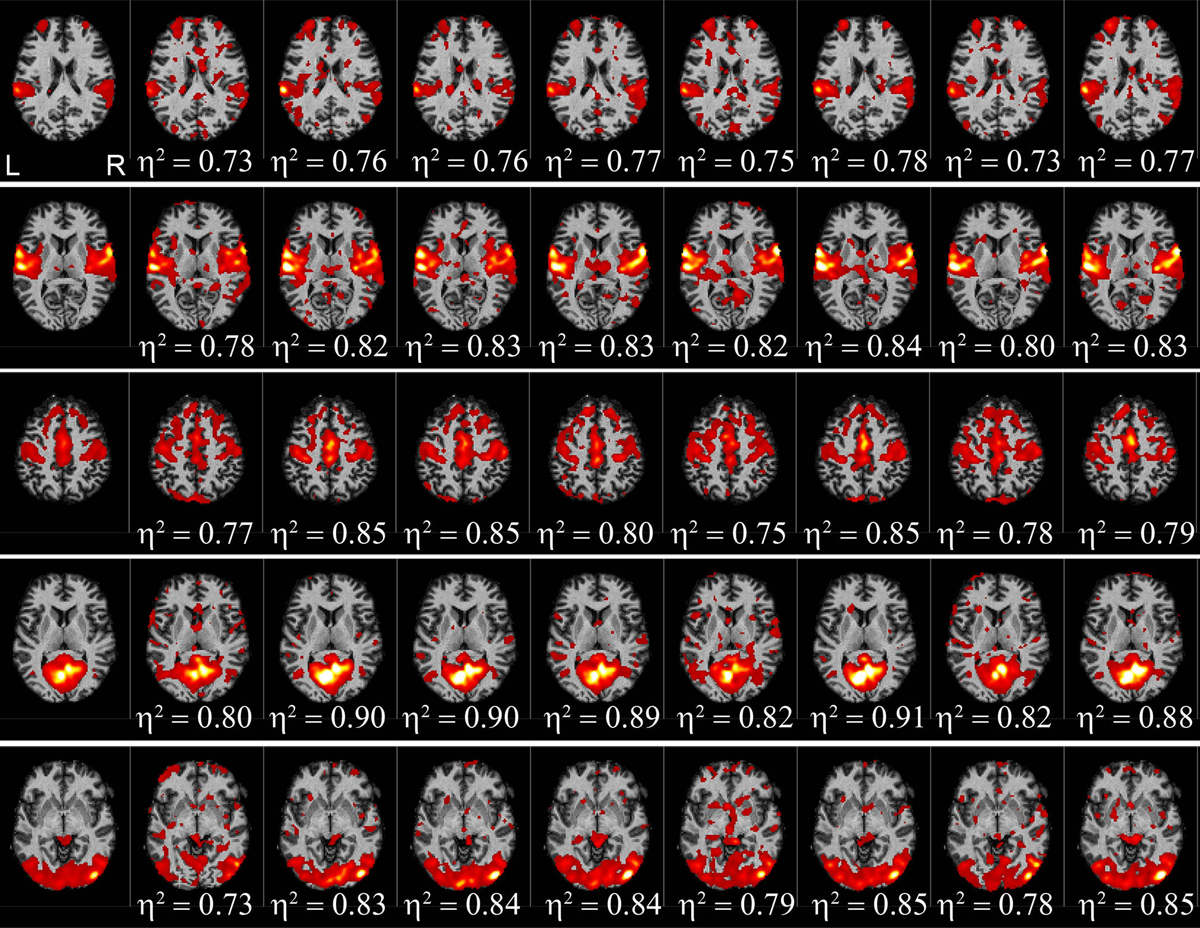
\includegraphics[width=\linewidth, height = 2.5in]{../DSC-H0217_03}
  \end{figure}
\end{frame}


\begin{frame} {Problems} 
\BIT
\item  multiple comparison problem - thousands of readings over time and space 
\item want to incorporate location and time information - want continuous significant regions, not voxels
\item want to determine these significant regions adaptively
\EIT
\end{frame}

\section{Method } 

\begin{frame} {The idea}
\BIT
\item focus on data with p-values rather than intensities
\item assume that data is generated according to a prior which induces clustering of significant p-values
\item get the posterior distribution (somehow) 
\item p-values which are in significant clusters are discoveries    
\EIT
\end{frame}


\begin{frame} {The prior we assumed}
\BIT
\item number of signal clusters:  $k \sim \mbox{Truncated Poisson}(\lambda,  1, k_{max})$
\item signal centers:   $c_j \sim \mbox{Uniform over location-time space}$ for $j = 1, ... , k$
\item signal radius:  $r_j \sim \mbox{Truncated Normal}(\mu,\sigma,r_{min},r_{max}) \mbox{ for j = 1, \ldots k} $.
\item signal strength:  $\beta_j \sim \mbox{Uniform}(\beta_{min},\beta_{max}) \mbox{ for j = 1, \ldots, k} $.
\item p-values in signal clusters:  $p_i \sim \mbox{Beta}(\frac{1}{\beta_j}, \beta_j)$, when $x_i$ is in cluster $j$.
\item p-values not in signal clusters:  $p_i \sim \mbox{Uniform}(0,1)$.
\EIT %note that this allows for overlapping clusters for biological reasons etc. 
\end{frame}
%comment on how crazy it is to sample from the prior

\begin{frame}{How do we write down the posterior??} 
\BIT
\item we don't - we sample from it
\item  we invented a Markov chain, inspired by Stephens (2000), with posterior distribution given by the likelihood of the data 
\item  the type of chain is a birth-death chain (over an infinite dimensional state space!)
\EIT 
\end{frame}

\begin{frame} {The rough algorithm}
\BIT 
\item initialize clusters and labels randomly by sampling from the prior 
\item  repeat the following 10,000 times
\BIT
\item flip a weighted coin to determine if a birth or death occurs
\item if birth, add a new cluster randomly 
\item if death, delete a cluster which doesn't explain the data well
\EIT
\item take the average of the last 5,000 labels to determine if a p-value is signal or null. 
\EIT 
\end{frame}


\section{Example: simulated data} 

\begin{frame} {Toy Data: Preliminaries}
\BIT
\item 100-by-100 grid with $k$=5 clusters of signals and the rest is null.
\item the centers $C_k \sim$  uniform from the grid while being distinct for $k = 1, 2, ..., 5$
\item the radius $R_k \sim T N (7, 2, 5, 10)$ for $k = 1, 2, ..., 5$
\item signals in clusters $p_{ki} \sim Beta(1, \beta_k)$ where $\beta_k \sim TN(8, 5, 2, 200)$ for $k = 1, 2, ..., 5$
\EIT
\end{frame}

\begin{frame} {Toy Data (continued): Performance }
\begin{figure}[t!]
    \centering
    \begin{subfigure}[t]{0.3\textwidth}
        \centering
        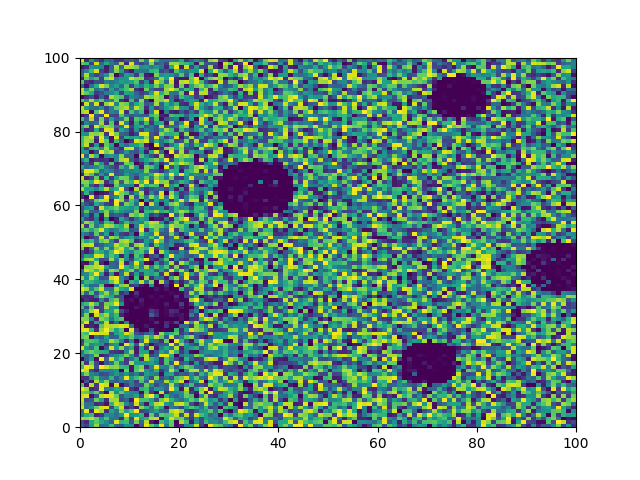
\includegraphics[height=1.2in, width=1.4in]{../BDC_gridactual}
        \caption{Actual grid}
    \end{subfigure}%
    \begin{subfigure}[t]{0.3\textwidth}
        \centering
        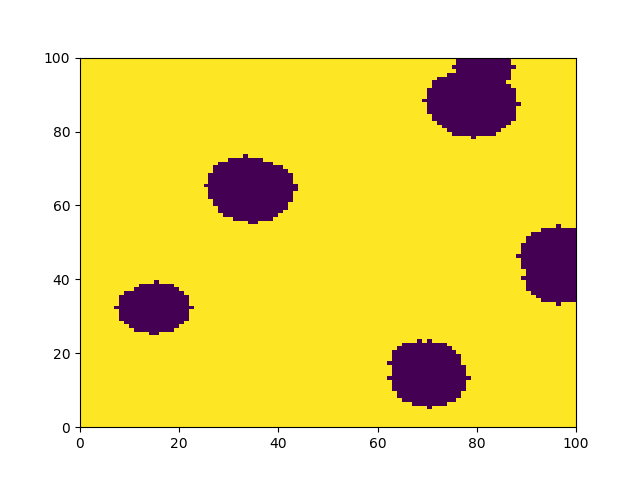
\includegraphics[height=1.2in, width=1.4in]{../BDC_grid1}
        \caption{Birth death chain}
    \end{subfigure}%
    \begin{subfigure}[t]{0.3\textwidth}
        \centering
        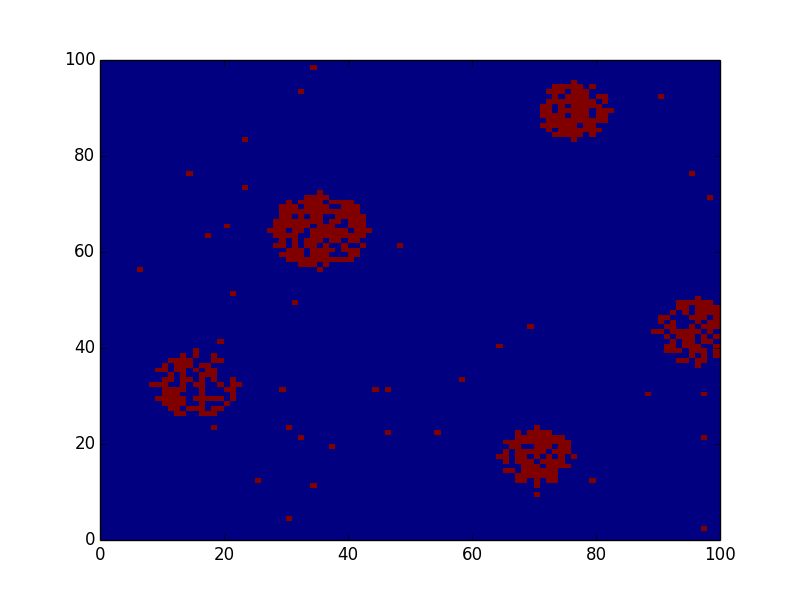
\includegraphics[height=1.2in, width=1.4in]{../BH_toy_data}
        \caption{BH}
    \end{subfigure}
    \caption{Simulated data}
\end{figure}
\end{frame}


\begin{frame}{Toy Data (continued): More on Priors}
\begin{figure}[t!]
    \centering
    \begin{subfigure}[t]{0.3\textwidth}
        \centering
        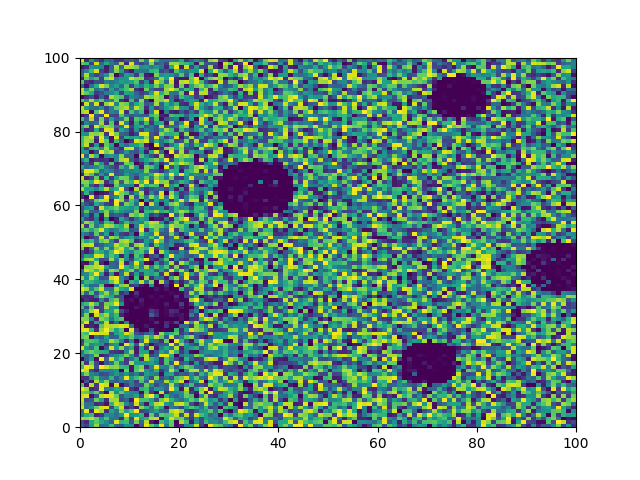
\includegraphics[height=1.2in, width=1.4in]{../BDC_gridactual}
        \caption{Actual grid}
    \end{subfigure}%
    \begin{subfigure}[t]{0.3\textwidth}
        \centering
        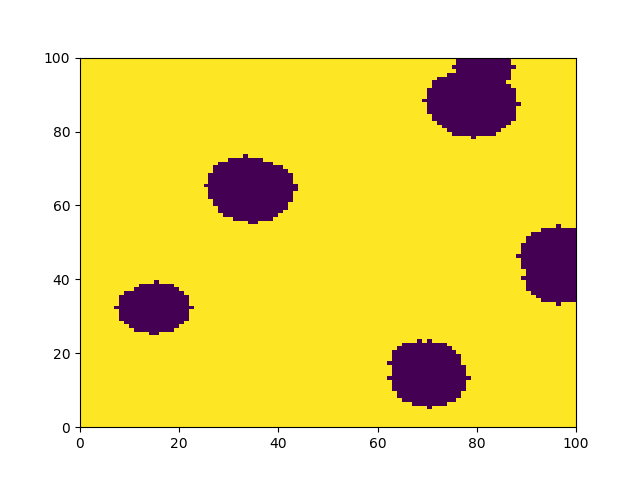
\includegraphics[height=1.2in, width=1.4in]{../BDC_grid1}
        \caption{$k \sim Trun(Poi(50), 1, 100)$; $r \sim TN(7, 2, 5, 10)$; $\beta \sim TN(8, 5, 2, 200)$}
    \end{subfigure} %
    \caption{Simulated data}
\end{figure}
\end{frame}


\begin{frame}{Toy Data (continued): More on Priors}
First, let's compare different priors on beta
\begin{figure}[t!]
    \centering
    \begin{subfigure}[t]{0.3\textwidth}
        \centering
        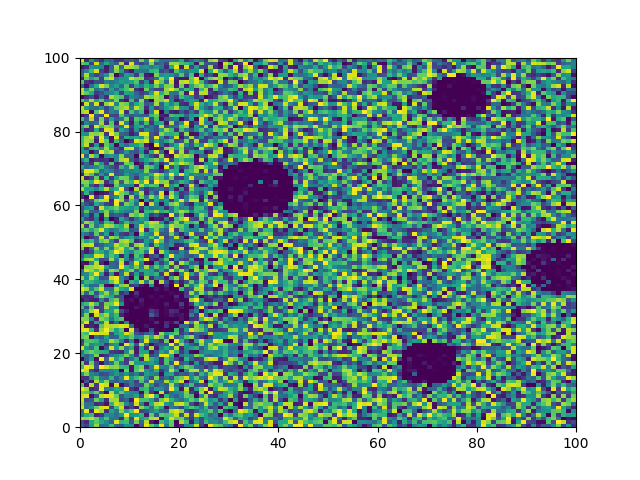
\includegraphics[height=1.3in, width=1.4in]{../BDC_gridactual}
        \caption{Actual grid}
    \end{subfigure}%
    \begin{subfigure}[t]{0.3\textwidth}
        \centering
        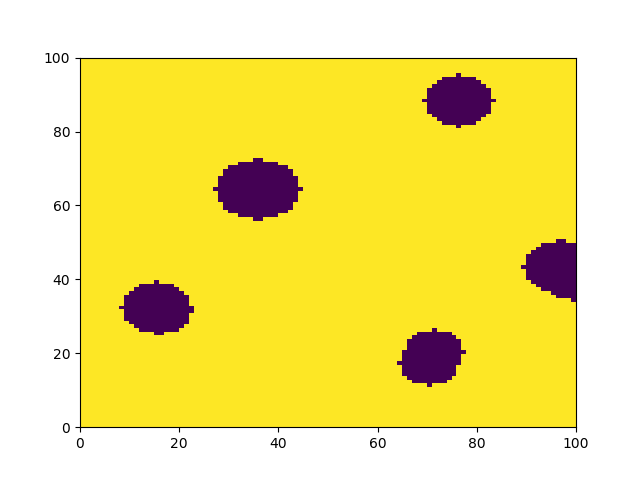
\includegraphics[height=1.2in, width=1.4in]{../BDC_grid2_strongsig}
        \caption{ $k \sim Trun(Poi(50), 1, 100)$; $r \sim TN(7, 2, 5, 10)$; $\beta \sim TN(30, 3, 2, 200)$}
    \end{subfigure}%
        \begin{subfigure}[t]{0.3\textwidth}
        \centering
        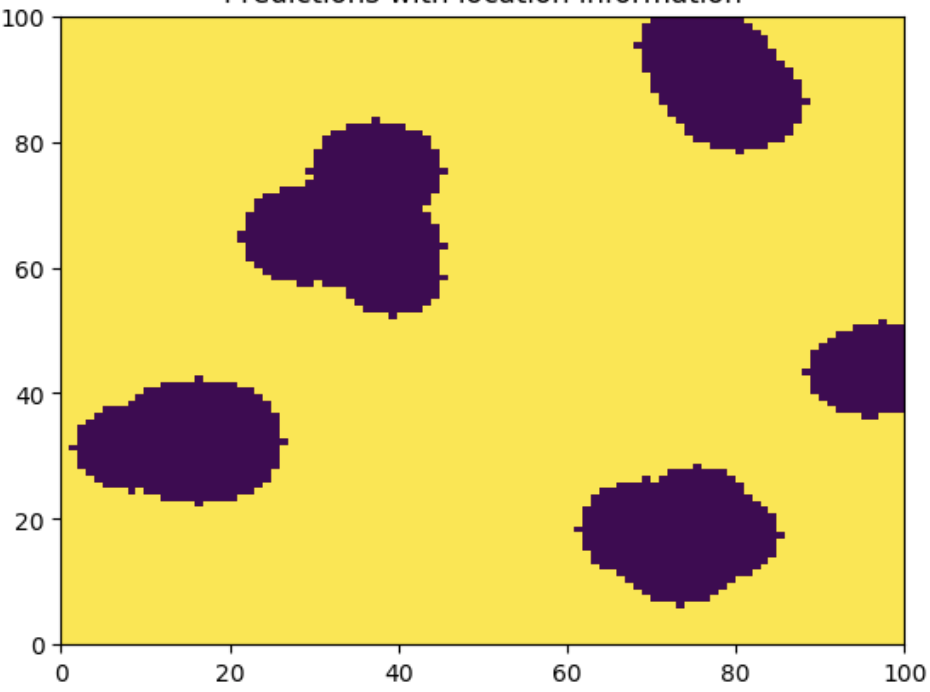
\includegraphics[height=1.2in, width=1.4in]{../BDC_grid3_weaksig}
        \caption{ $k \sim Trun(Poi(50), 1, 100)$; $r \sim TN(7, 2, 5, 10)$; \textbf{$\beta \sim TN(2, 1, 2, 200)$}}
    \end{subfigure}
    \caption{Simulated data}
\end{figure}
\end{frame}

\begin{frame}{Toy Data (continued): More on Priors}
Now, let's compare different priors on radius.
\begin{figure}[t!]
    \centering
    \begin{subfigure}[t]{0.3\textwidth}
        \centering
        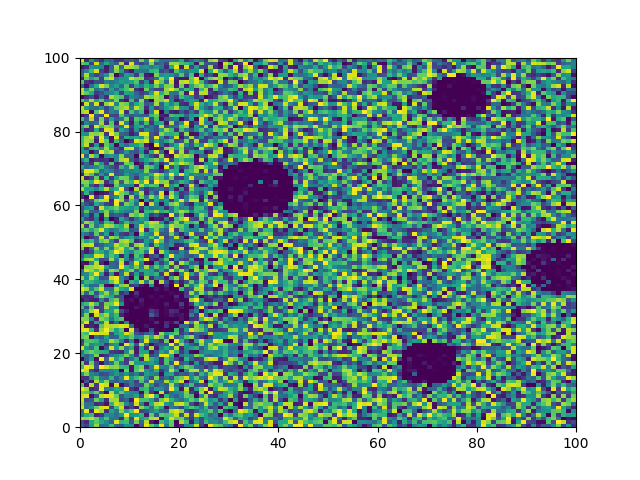
\includegraphics[height=1.3in, width=1.4in]{../BDC_gridactual}
        \caption{Actual grid}
    \end{subfigure}%
    \begin{subfigure}[t]{0.3\textwidth}
        \centering
        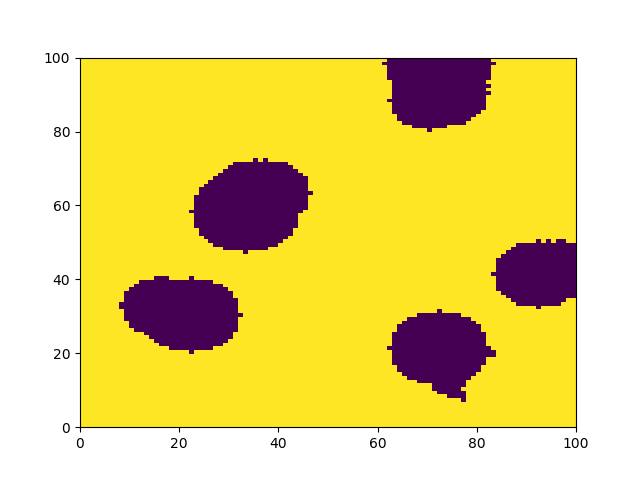
\includegraphics[height=1.2in, width=1.4in]{../BDC_grid4}
        \caption{ $k \sim Trun(Poi(50), 1, 100)$; $r \sim TN(10, 2, 7, 13)$; $\beta \sim TN(8, 5, 2, 200)$}
    \end{subfigure}%
        \begin{subfigure}[t]{0.3\textwidth}
        \centering
        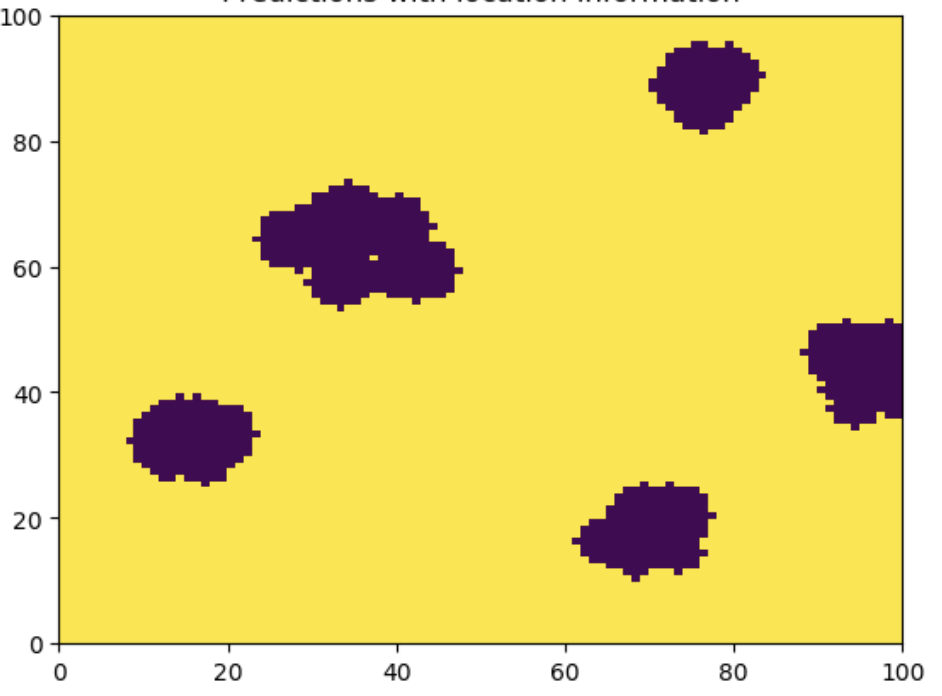
\includegraphics[height=1.2in, width=1.4in]{../BDC_grid5}
        \caption{ $k \sim Trun(Poi(50), 1, 100)$; $r \sim TN(2, 2, 1, 10)$; $\beta \sim TN(8, 5, 2, 200)$}
    \end{subfigure}
    \caption{Simulated data}
\end{figure}
\end{frame}


\begin{frame}{Toy Data (continued): More on Priors}
What if we make signal stronger?
\begin{figure}[t!]
    \centering
    \begin{subfigure}[t]{0.3\textwidth}
        \centering
        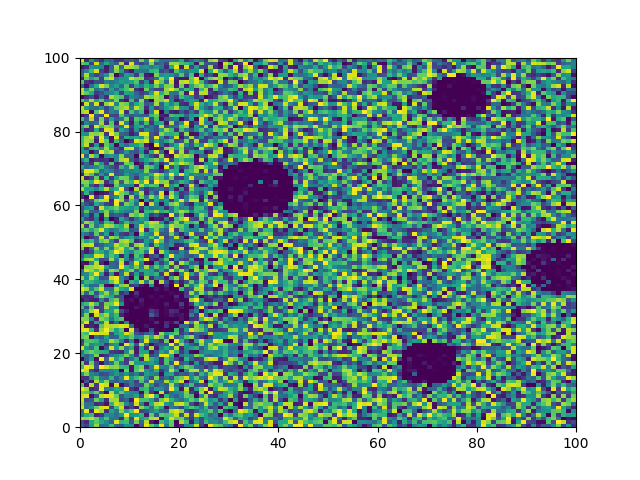
\includegraphics[height=1.3in, width=1.4in]{../BDC_gridactual}
        \caption{Actual grid}
    \end{subfigure}%
    \begin{subfigure}[t]{0.3\textwidth}
        \centering
        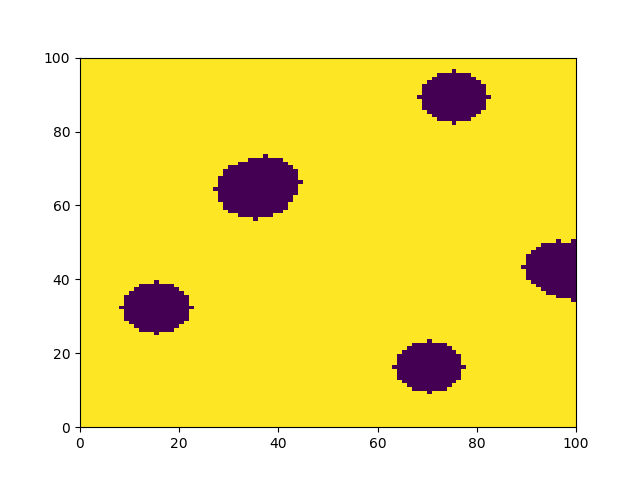
\includegraphics[height=1.2in, width=1.4in]{../BDC_grid4_bigradius_ss}
        \caption{ $k \sim Trun(Poi(50), 1, 100)$; $r \sim TN(10, 2, 7, 13)$; $\beta \sim TN(30, 3, 2, 200)$}
    \end{subfigure}%
        \begin{subfigure}[t]{0.3\textwidth}
        \centering
        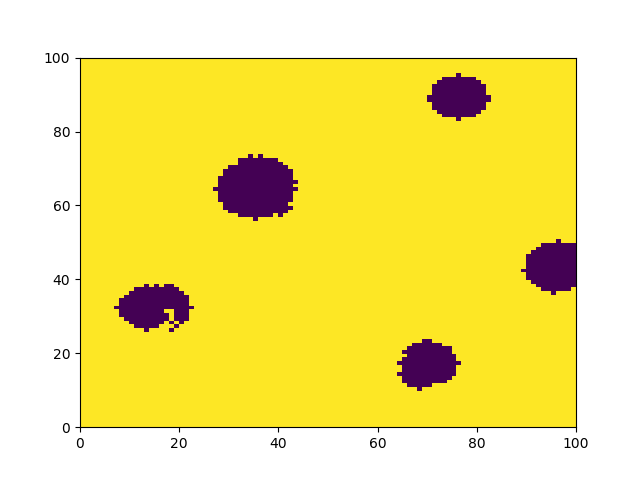
\includegraphics[height=1.2in, width=1.4in]{../BDC_grid5_smallradius_ss}
        \caption{ $k \sim Trun(Poi(50), 1, 100)$; $r \sim TN(2, 2, 1, 10)$; $\beta \sim TN(30, 3, 2, 200)$}
    \end{subfigure}
    \caption{Simulated data}
\end{figure}
\end{frame}


\begin{frame}{Toy Data (continued): More on Priors}
Next, we change the priors on number of clusters.
\begin{figure}[t!]
    \centering
    \begin{subfigure}[t]{0.3\textwidth}
        \centering
        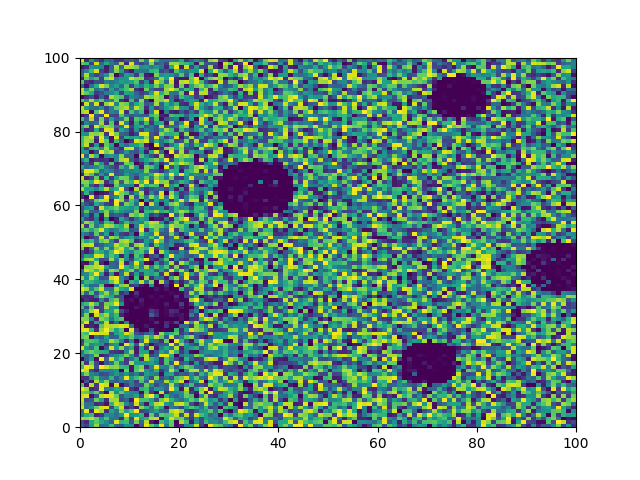
\includegraphics[height=1.3in, width=1.4in]{../BDC_gridactual}
        \caption{Actual grid}
    \end{subfigure}%
    \begin{subfigure}[t]{0.3\textwidth}
        \centering
        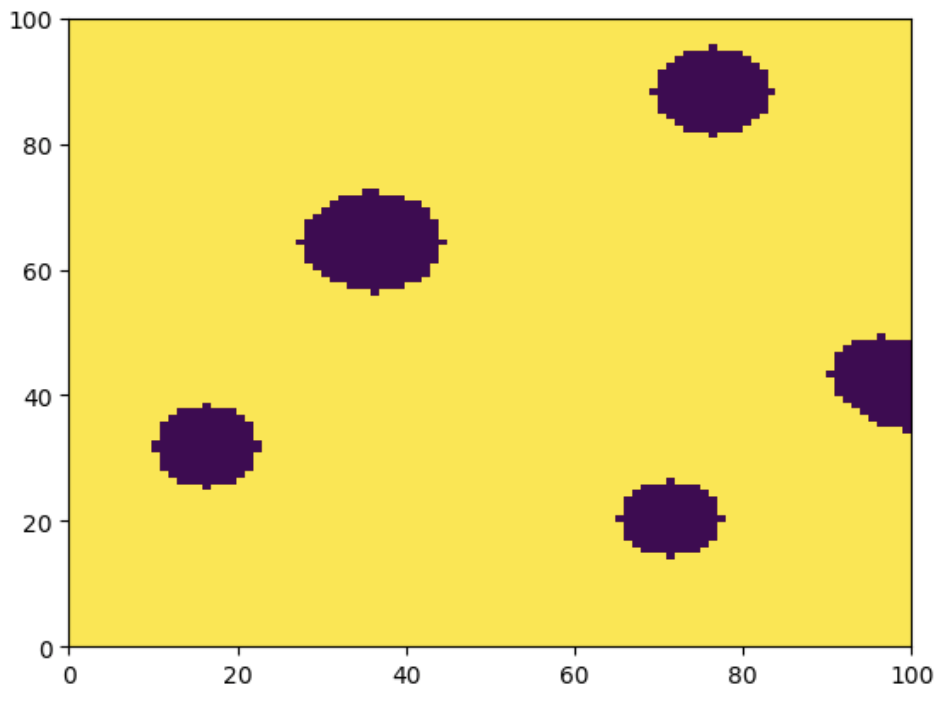
\includegraphics[height=1.2in, width=1.4in]{../BDC_grid7_c3}
        \caption{ $k \sim Trun(Poi(3), 1, 10)$; $r \sim TN(7, 2, 5, 10)$; $\beta \sim TN(8, 5, 2, 200)$}
    \end{subfigure}%
        \begin{subfigure}[t]{0.3\textwidth}
        \centering
        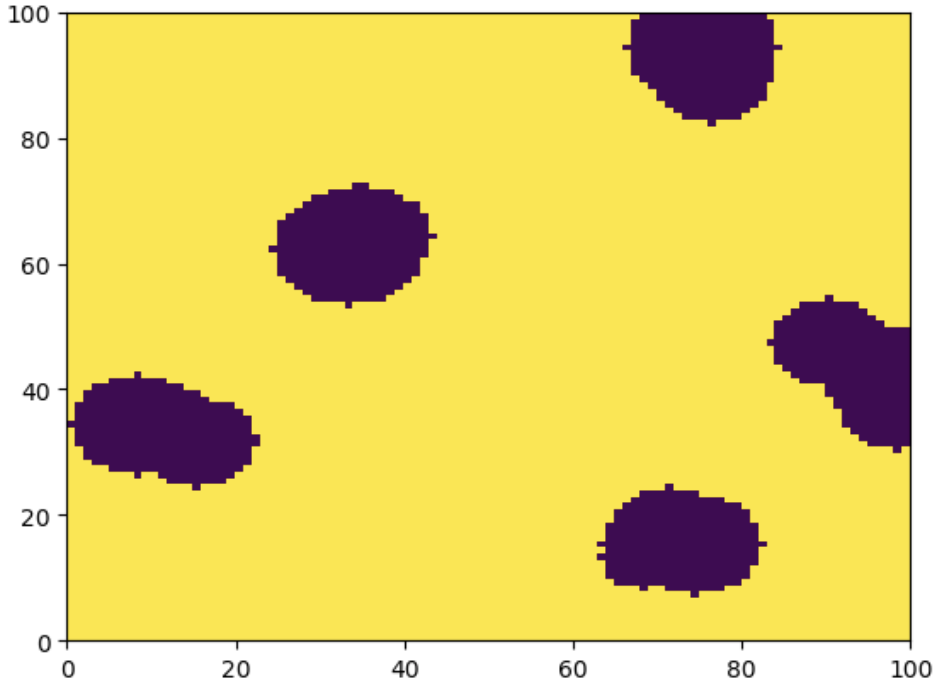
\includegraphics[height=1.2in, width=1.4in]{../BDC_grid8_c300}
        \caption{ $k \sim Trun(Poi(300), 1, 1000)$; $r \sim TN(7, 2, 5, 10)$; $\beta \sim TN(8, 5, 2, 200)$}
    \end{subfigure}
    \caption{Simulated data}
\end{figure}
\end{frame}


\begin{frame}{Toy Data (continued): More on Priors}
Again, let's make signal stronger
\begin{figure}[t!]
    \centering
    \begin{subfigure}[t]{0.3\textwidth}
        \centering
        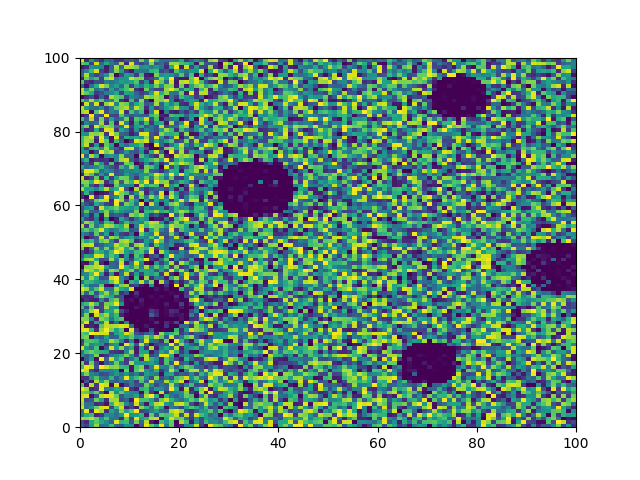
\includegraphics[height=1.3in, width=1.4in]{../BDC_gridactual}
        \caption{Actual grid}
    \end{subfigure}%
    \begin{subfigure}[t]{0.3\textwidth}
        \centering
        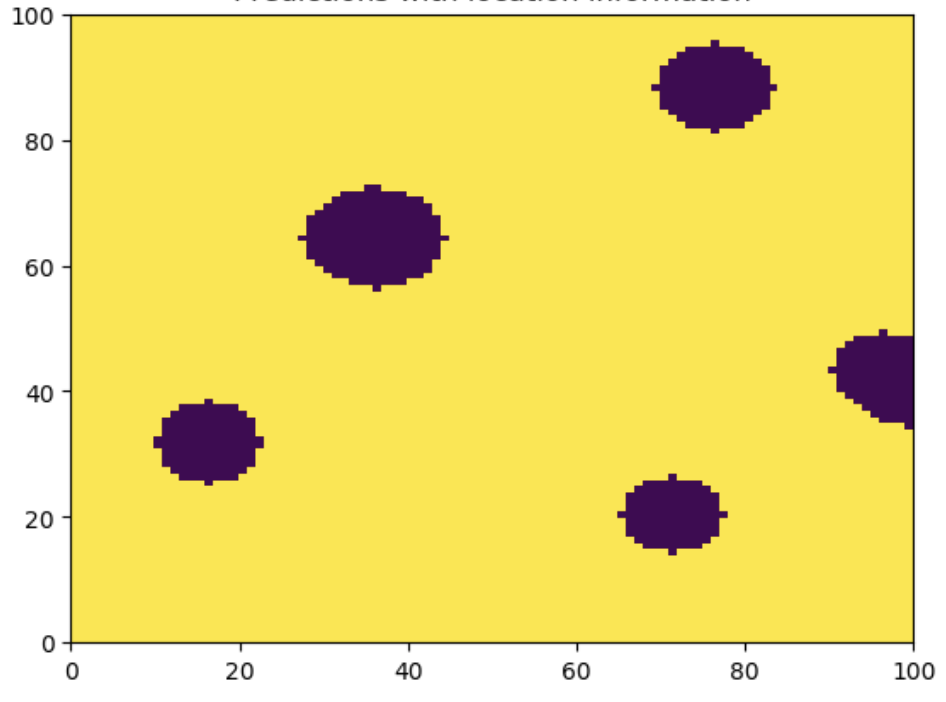
\includegraphics[height=1.2in, width=1.4in]{../BDC_grid7_c3_ss}
        \caption{ $k \sim Trun(Poi(3), 1, 10)$; $r \sim TN(7, 2, 5, 10)$; $\beta \sim TN(30, 3, 2, 200)$}
    \end{subfigure}%
        \begin{subfigure}[t]{0.3\textwidth}
        \centering
        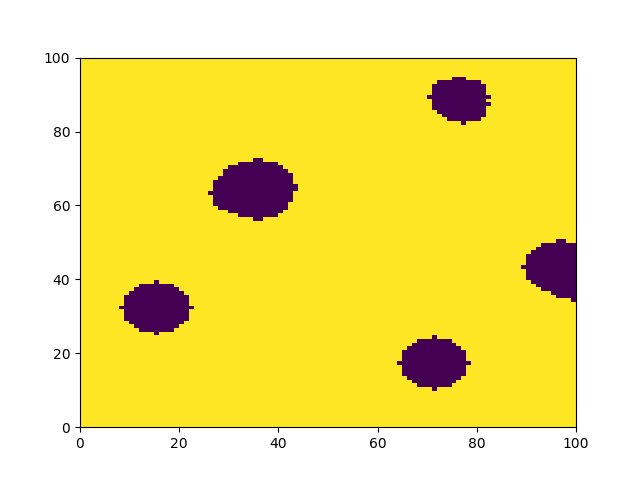
\includegraphics[height=1.2in, width=1.4in]{../BDC_grid8_c300_ss}
        \caption{ $k \sim Trun(Poi(300), 1, 1000)$; $r \sim TN(7, 2, 5, 10)$; $\beta \sim TN(30, 3, 2, 200)$}
    \end{subfigure}
    \caption{Simulated data}
\end{figure}
\end{frame}


\begin{frame}{Toy Data 2 (3-D)}
\begin{figure}[t!]
    \centering
    \begin{subfigure}[t]{0.3\textwidth}
        \centering
        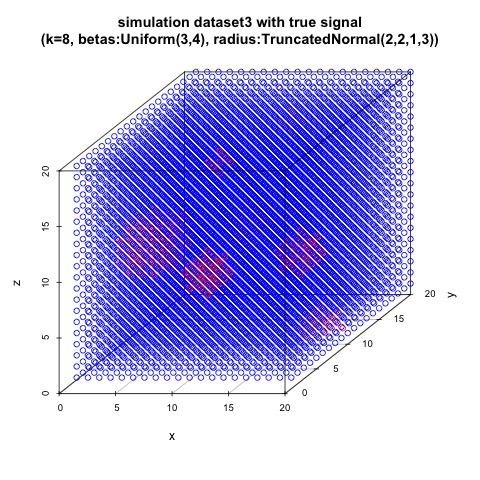
\includegraphics[height=1.4in, width=1.4in]{../simulation_data3.jpg}
        \caption{}
    \end{subfigure}%
    \begin{subfigure}[t]{0.3\textwidth}
        \centering
        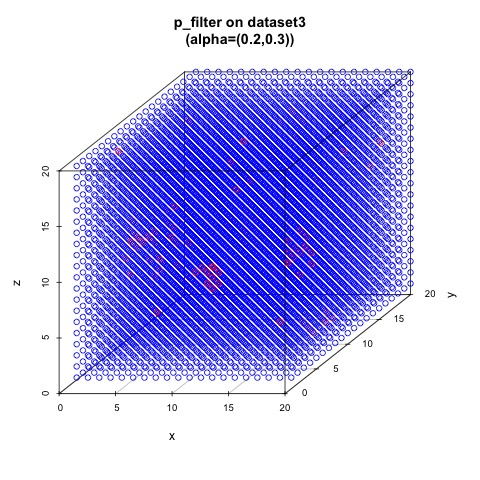
\includegraphics[height=1.4in, width=1.4in]{../p_filterondataset3.jpg}
        \caption{}
    \end{subfigure}%
        \begin{subfigure}[t]{0.3\textwidth}
        \centering
        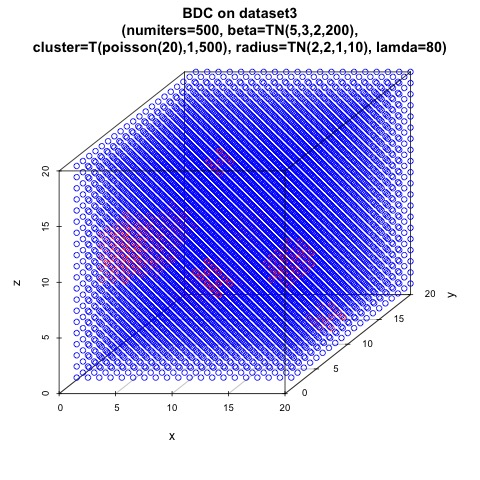
\includegraphics[height=1.4in, width=1.4in]{../best3.jpg}
        \caption{}
    \end{subfigure}
    \caption{Simulated data}
\end{figure}
\end{frame}


\begin{frame}{Toy Data 2 (3-D)}
\begin{figure}[t!]
    \centering
    \begin{subfigure}[t]{0.3\textwidth}
        \centering
        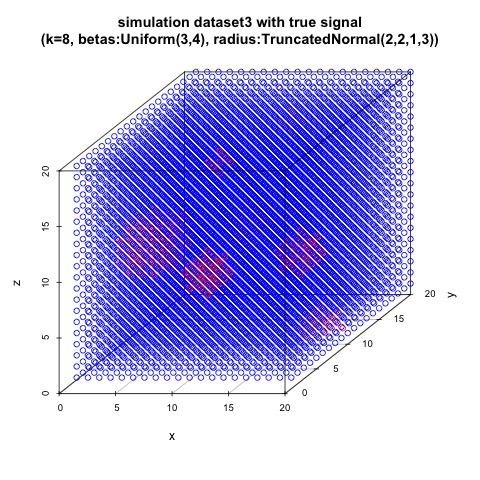
\includegraphics[height=1.4in, width=1.4in]{../simulation_data3.jpg}
        \caption{}
    \end{subfigure}%
    \begin{subfigure}[t]{0.3\textwidth}
        \centering
        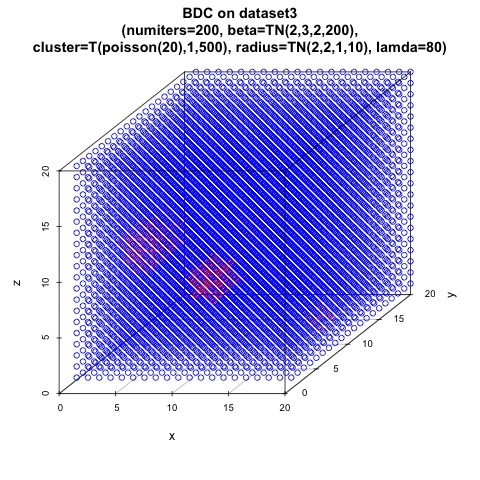
\includegraphics[height=1.4in, width=1.4in]{../dataset3beta3.jpg}
        \caption{}
    \end{subfigure}%
        \begin{subfigure}[t]{0.3\textwidth}
        \centering
        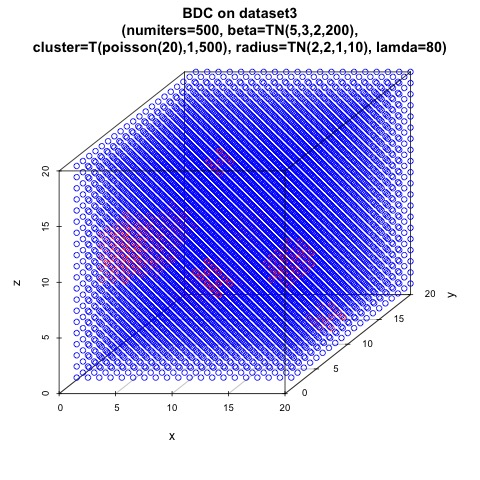
\includegraphics[height=1.4in, width=1.4in]{../best3.jpg}
        \caption{}
    \end{subfigure}
    \caption{Simulated data}
\end{figure}
\end{frame}

\begin{frame}{Toy Data 2 (3-D)}
\begin{figure}[t!]
    \centering
    \begin{subfigure}[t]{0.3\textwidth}
        \centering
        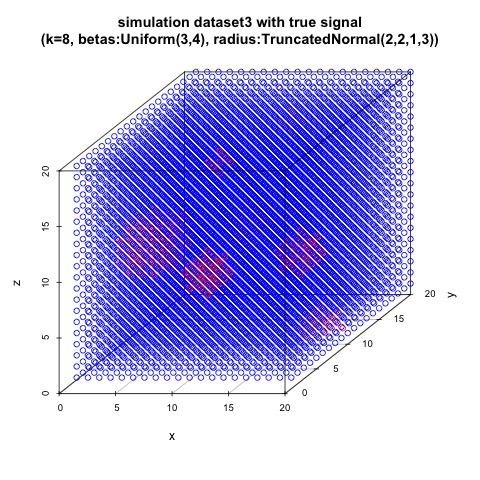
\includegraphics[height=1.4in, width=1.4in]{../simulation_data3.jpg}
        \caption{}
    \end{subfigure}%
    \begin{subfigure}[t]{0.3\textwidth}
        \centering
        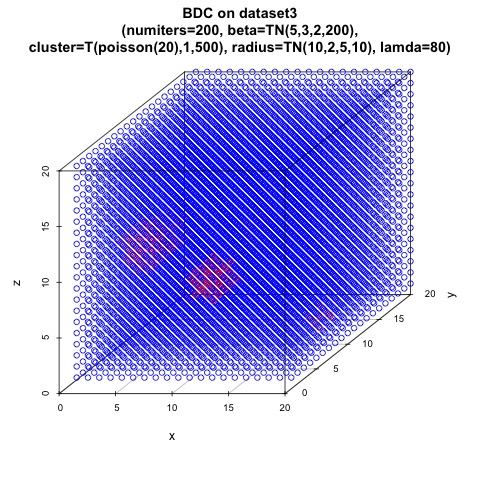
\includegraphics[height=1.4in, width=1.4in]{../radius10.jpg}
        \caption{}
    \end{subfigure}%
        \begin{subfigure}[t]{0.3\textwidth}
        \centering
        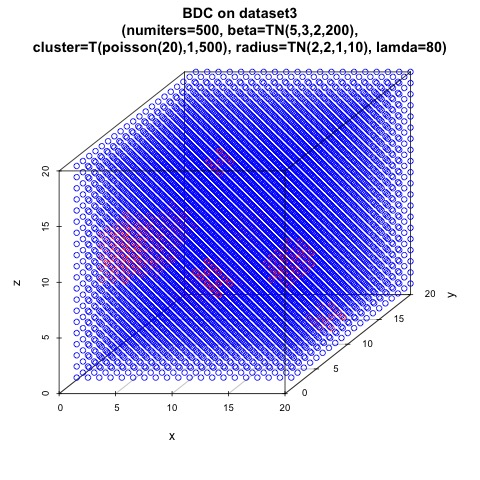
\includegraphics[height=1.4in, width=1.4in]{../best3.jpg}
        \caption{}
    \end{subfigure}
    \caption{Simulated data}
\end{figure}
\end{frame}


\begin{frame}{Toy Data 2 (3-D)}
\begin{figure}[t!]
    \centering
    \begin{subfigure}[t]{0.3\textwidth}
        \centering
        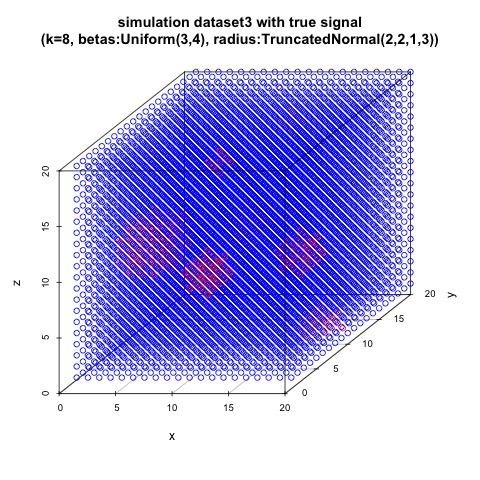
\includegraphics[height=1.4in, width=1.4in]{../simulation_data3.jpg}
        \caption{}
    \end{subfigure}%
    \begin{subfigure}[t]{0.3\textwidth}
        \centering
        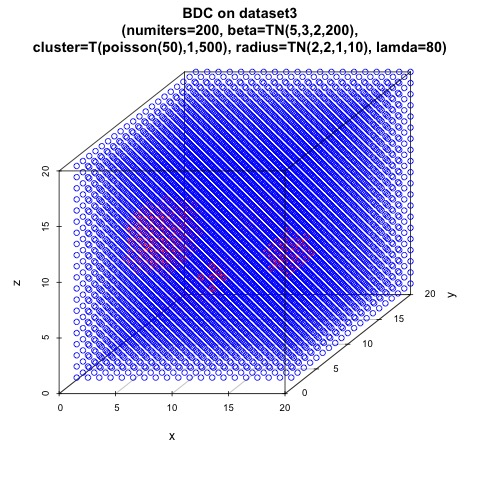
\includegraphics[height=1.4in, width=1.4in]{../datase3_poi50.jpg}
        \caption{}
    \end{subfigure}%
        \begin{subfigure}[t]{0.3\textwidth}
        \centering
        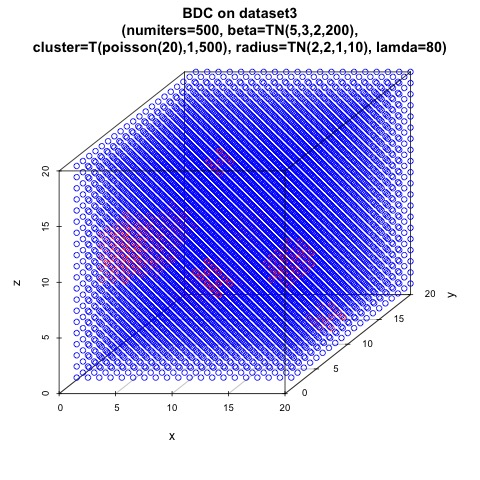
\includegraphics[height=1.4in, width=1.4in]{../best3.jpg}
        \caption{}
    \end{subfigure}
    \caption{Simulated data}
\end{figure}
\end{frame}

\begin{frame}{Conclusion and Future Work}
\BIT
\item presented a nonparametric-bayesian method to adaptively identify clusters of signals.
\item it showed promising results on both simulation and real fMRI data.
\item possible extensions
\BIT 
\item work with intensities directly by specifying appropriate priors for null distributions and for signal distributions.
\item put priors on the hyper-parameters and maximize these priors using EM
\EIT  
\EIT
\begin{center}
\textbf{\large Thanks!}
\end{center}
\end{frame}


\end{document}
